\documentclass[11pt,a4paper,onecolumn]{article}
\usepackage[T1]{fontenc}
\usepackage[utf8]{inputenc}
\usepackage{lmodern,microtype}
\usepackage[margin=1in]{geometry}
\usepackage{amsmath,amssymb,amsthm,mathtools}
\usepackage{booktabs,tabularx,array,enumitem}
\usepackage{float}
\usepackage{needspace}
\usepackage[section]{placeins}
\usepackage{tikz}
\usetikzlibrary{arrows.meta}
\usepackage[framemethod=default]{mdframed}
\usepackage{xcolor}
\usepackage[hidelinks]{hyperref}
\hypersetup{pdftitle={An L1-Authorized Sequencing Service with Regional Failover},
pdfsubject={Proposed protocol: model, algorithms, proofs and complexity}}
\usepackage[nameinlink,noabbrev]{cleveref}
\usepackage{fancyhdr}
\setlength{\headheight}{14pt}
\pagestyle{fancy}\fancyhf{}
\lhead{\small An authorized sequencing service}\rhead{\small Proposed protocol}
\cfoot{\thepage}
\setlength{\emergencystretch}{2em}
\setlist{nosep,leftmargin=*}
\newcolumntype{Y}{>{\raggedright\arraybackslash}X}
\newcommand{\Hash}{\mathsf H}
\newcommand{\Sig}{\mathsf{Sign}}
\newcommand{\Ver}{\mathsf{Verify}}
\newcommand{\QC}{\mathsf{QC}}
\newcommand{\RC}{\mathsf{RC}}
\newcommand{\Cfg}{\mathsf{Cfg}}
\newcommand{\gv}{v_{\mathrm G}}
\newcommand{\lv}{v_{\mathrm L}}
\newcommand{\BB}{\mathsf{BB}}
\newcommand{\AB}{\mathsf{AB}}
\newcommand{\BA}{\mathsf{BA}}
\newcommand{\botv}{\bot}
\newcommand{\pre}{\preceq}
\newcommand{\wt}{\operatorname{wt}}
\newcommand{\id}{\operatorname{id}}
\newcommand{\tip}{\operatorname{tip}}
\newcommand{\parh}{\operatorname{parent}}
\newcommand{\Tag}[1]{\mathsf{#1}}
\newcommand{\Proc}[1]{\textnormal{\textsc{#1}}}
\newtheorem{definition}{Definition}[section]
\newtheorem{assumption}[definition]{Assumption}
\newtheorem{lemma}[definition]{Lemma}
\newtheorem{theorem}[definition]{Theorem}
\newtheorem{proposition}[definition]{Proposition}
\theoremstyle{remark}\newtheorem{example}[definition]{Example}
\newtheorem{remark}[definition]{Remark}
\newcounter{protocol}
\newenvironment{protocol}[2]{\refstepcounter{protocol}\label{#1}\begin{mdframed}[nobreak=true,linewidth=.6pt,skipabove=10pt,skipbelow=10pt,innertopmargin=8pt,innerbottommargin=8pt]\small\raggedright\noindent\textbf{Protocol \theprotocol. #2}\par\smallskip}{\end{mdframed}}
\crefname{protocol}{Protocol}{Protocols}
\Crefname{protocol}{Protocol}{Protocols}
\crefname{definition}{Definition}{Definitions}
\crefname{assumption}{Assumption}{Assumptions}
\crefname{lemma}{Lemma}{Lemmas}
\crefname{theorem}{Theorem}{Theorems}
\crefname{proposition}{Proposition}{Propositions}
\title{An L1-Authorized Sequencing Service with Regional Failover\\
\large A Proposed Protocol for Verifiable Mini-Block Streams}
\author{}\date{25 September 2026}
\begin{document}
\begin{center}
{\Large\bfseries An L1-Authorized Sequencing Service\\with Regional Failover\par}
\vspace{.5em}
{\normalsize A Proposed Protocol for Verifiable Mini-Block Streams\par}
\vspace{.4em}{\small 25 September 2026}
\end{center}
\begin{abstract}
We specify an L1-authorized sequencing service whose producer rotates within
and between geographic regions. Regional broadcast yields fast previews;
explicit global agreement and FFG links yield durable delivery and geographic
activation. Producer push, peer pull and a cross-region backbone separate data
transport from confirmation. We give complete protocols, illustrative traces,
agreement and verification proofs, and latency and communication bounds for
normal service, local faults and regional outages. This is a proposed protocol;
consumer execution and publication lie outside its interface.
\end{abstract}

\section{Introduction}\label{sec:intro}
The purpose of the service is to deliver a continuous, verifiable transaction
stream under L1-authorized production rights. At any time one geographic region
is active, and one sequencer in that region produces ordered mini-blocks.
A local failure transfers production to another regional member; a regional
outage transfers it to another region. A proposer consumes the stream through
the same interface before and after these changes. 

\begin{figure}[H]\centering
% Native TikZ input for main_v1.tex. Shared earlier-version figures are unchanged.
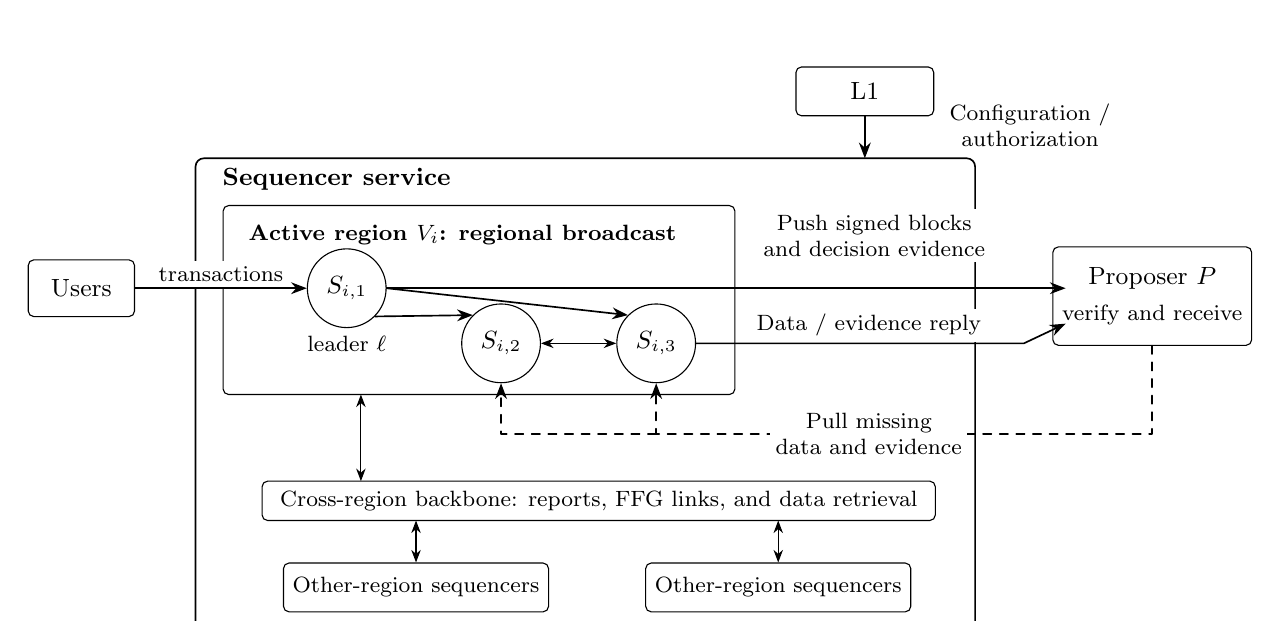
\begin{tikzpicture}[
  x=1cm,y=1cm,font=\small,line cap=round,line join=round,
  archbox/.style={draw,rounded corners=2pt,align=center,fill=white},
  archseq/.style={draw,circle,minimum size=10mm,inner sep=1pt,fill=white},
  archflow/.style={-{Stealth[length=2mm]},semithick},
  archpull/.style={-{Stealth[length=2mm]},semithick,dashed},
  archcontrol/.style={{Stealth[length=1.6mm]}-{Stealth[length=1.6mm]},thin},
  archlabel/.style={font=\footnotesize,fill=white,inner sep=2pt,align=center}
]
  \draw[rounded corners=3pt,semithick] (2.20,0) rectangle (12.10,6.00);
  \node[anchor=west,font=\small\bfseries] at (2.42,5.73) {Sequencer service};
  \draw[rounded corners=2pt] (2.55,3.00) rectangle (9.05,5.40);
  \node[anchor=north west,font=\footnotesize\bfseries] at (2.75,5.28)
    {Active region $V_i$: regional broadcast};

  \node[archbox,minimum width=1.35cm,minimum height=.72cm] (users) at (.75,4.35)
    {Users};
  \node[archseq] (leader) at (4.12,4.35) {$S_{i,1}$};
  \node[archlabel,anchor=north] at (4.12,3.82) {leader $\ell$};
  \node[archseq] (peerone) at (6.08,3.65) {$S_{i,2}$};
  \node[archseq] (peertwo) at (8.05,3.65) {$S_{i,3}$};
  \draw[archflow] (leader.south east) -- (peerone.north west);
  \draw[archflow] (leader.east) -- (peertwo.north west);
  \draw[archcontrol] (peerone.east) -- (peertwo.west);
  \draw[archflow] (users.east) -- node[archlabel,above] {transactions} (leader.west);

  \node[archbox,minimum width=2.20cm,minimum height=1.25cm] (consumer) at (14.35,4.25)
    {Proposer $P$\\[2pt]\footnotesize verify and receive};
  \draw[archflow] (leader.east) -- (13.25,4.35);
  \node[archlabel] at (10.82,5.02) {Push signed blocks\\and decision evidence};
  \draw[archpull] (14.35,3.62) -- (14.35,2.50) -- (8.05,2.50) -- (peertwo.south);
  \draw[archpull] (8.05,2.50) -- (6.08,2.50) -- (peerone.south);
  \node[archlabel] at (10.75,2.50) {Pull missing\\data and evidence};
  \draw[archflow] (peertwo.east) -- (12.72,3.65) -- (13.25,3.90);
  \node[archlabel] at (10.75,3.88) {Data / evidence reply};

  \node[archbox,minimum width=8.55cm,minimum height=.50cm] (backbone) at (7.32,1.65)
    {\footnotesize Cross-region backbone: reports, FFG links, and data retrieval};
  \draw[archcontrol] (4.30,3.00) -- (4.30,1.90);
  \node[archbox,minimum width=2.80cm,minimum height=.62cm] (regiontwo) at (5.00,.55)
    {\footnotesize Other-region sequencers};
  \node[archbox,minimum width=2.80cm,minimum height=.62cm] (regionthree) at (9.60,.55)
    {\footnotesize Other-region sequencers};
  \draw[archcontrol] (5.00,1.40) -- (regiontwo.north);
  \draw[archcontrol] (9.60,1.40) -- (regionthree.north);

  \node[archbox,minimum width=1.75cm,minimum height=.62cm] (lone) at (10.70,6.85) {L1};
  \draw[archflow] (lone.south) -- (10.70,6.00);
  \node[archlabel,anchor=west] at (11.70,6.42) {Configuration /\\authorization};
\end{tikzpicture}

\caption{The sequencing service and its external interfaces. The three drawn
sequencers illustrate communication roles; committee sizes and fault bounds
are specified in Section~\ref{sec:model}. A three-member equal-weight committee
under a strict one-third bound tolerates no Byzantine member.}
\label{fig:architecture}
\end{figure}

The active region confirms ordered mini-block batches; consumers receive leader
pushes and repair gaps by pulling from regional peers. Backbone synchronization
supplies the data and reports for global checkpoints. Local view changes preserve
the regional certified prefix. Geographic changes retain the global control
prefix, including every finalized delivery, and discard only its unretained
preview tail. A concrete synchronous report protocol precedes FFG voting,
making convergence and finality explicit.

\section{System Model and Setup}\label{sec:model}
\subsection{Participants and L1 authorization}
The sequencers form a fixed set $V=\biguplus_{i=1}^{m}V_i$, partitioned into
regions. Write $S_{i,j}\in V_i$, $n_i=|V_i|$, and $N=|V|$. Each sequencer $S$
has voting weight $w_S>0$. For $U\subseteq V$,
\[
 \wt(U)=\sum_{S\in U}w_S,\qquad W_i=\wt(V_i),\qquad W=\wt(V).
\]
A quorum of committee $Q$ contains distinct members of total weight
$>2\wt(Q)/3$. Clients submit transactions to the current leader, which selects
and orders them. $P$ denotes an external proposer consuming the stream.

L1 installs a fixed configuration
\begin{equation}\label{eq:cfg}
 \Cfg_c=(c,V,\{V_i\},w,\mathcal L,\Theta,G_0),
\end{equation}
consisting of:
\begin{itemize}
\item \textbf{Identity and membership:} the chain/configuration identifier $c$,
sequencers $V$, regional partition $\{V_i\}$, and voting weights $w$.
\item \textbf{Schedules:} $\mathcal L$ contains cyclic local leader lists and a
cyclic region list, each listing its members exactly once.
\item \textbf{Parameters:} $\Theta$ fixes timing and object-size limits,
including \eqref{eq:spacing}, the epoch budget of \cref{alg:global}, and the
complete-outcome admission limits of \cref{sec:latency}. Count limits and
rotation thresholds are positive integers; time and byte budgets are positive.
\item \textbf{Genesis:} $G_0$ fixes the initial active region, stream tip and
justified/finalized genesis checkpoint.
\end{itemize}
L1 delegates authority through the protocol's certified local rotations and
finalized global view changes, including recovery in the same region. These
transitions require no new L1 transaction; membership, weights and rules remain
fixed within a configuration.

\subsection{Established interfaces}
The setup provides authenticated identities and the following interfaces:
\begin{itemize}
\item \textbf{Communication:} $\Tag{Send}_{S\to T}(m)$ transmits $m$ over an
authenticated point-to-point channel from $S$ to $T$.
\item \textbf{Signatures:} $\Sig_S(m)$ produces a transferable signature;
$\Ver_S(m,\sigma)\in\{0,1\}$ checks it. Honest signatures cannot be forged.
\item \textbf{Commitments:} $\Hash(x)$ returns a binding digest of a canonically
encoded tuple or ordered list.
\end{itemize}
Every signed statement binds its configuration, message type and instance.
Canonical encoding distinguishes tuples, lists, integers, digests and byte
strings, and includes list lengths and element boundaries. In an expression
such as $\Hash(\Tag{TXLIST},\mathcal X)$, the uppercase word is a fixed
\emph{type tag}, encoded together with the arguments to separate message
domains; $\mathcal X$ is the data being committed to. Tags are not variables.

\subsection{Communication and time}\label{sec:network}
A common logical clock fixes synchronized instance starts. Complete protocol
objects travel between responsive honest nodes within $\Delta_R$ in a live
region and $\Delta_G$ across regions; actual regional delay is
$\delta_R\leq\Delta_R$. These bounds cover payload retrieval, transmission,
verification and queueing for all prescribed honest traffic within the configured
admission limits.


\subsection{Honesty and availability}
\begin{assumption}[Honest supermajorities]\label[assumption]{ass:env}
The Byzantine set $B\subseteq V$ is fixed during a configuration. Each region has honest
weight $\wt(V_i\setminus B)>2W_i/3$, and historical honest keys remain uncompromised.
\end{assumption}
Byzantine nodes may deviate arbitrarily.

Availability is specified separately:
\begin{itemize}
\item \textbf{Global envelope:} an honest set $H_G$ remains responsive
throughout the analyzed execution, with $\wt(H_G)>2W/3$.
\item \textbf{Live regional interval:} an honest set $H_i\subseteq V_i$ remains
responsive throughout the instance and its completion, with $\wt(H_i)>2W_i/3$.
\end{itemize}
Responsiveness includes meeting the communication bounds above.
A live consumer has a responsive data path to retained honest holders and
finite complete-object transfer and verification deadlines; the consumer-path
delays are accounted for separately in \cref{sec:latency}.
A \emph{healthy eligible successor} $j$ satisfies
$\wt(H_G\cap V_j)>2W_j/3$ and the regional communication bound on that set;
it may be the recovered current region. Whole-region outages are handled by
$H_G$ and such a successor. Progress further requires the workload, retrieval
and minimum-tenure conditions of \cref{sec:latency}.

\Needspace{18\baselineskip}
\subsection{Views, epochs, and block heights}\label{sec:indices}
The protocol has two levels of views. A \emph{global view} $\gv$ authorizes one
region $V_i$ to provide the stream. Within it, a \emph{local view} $\lv$ fixes
the leader $\ell\in V_i$. Thus $(\gv,\lv)$ identifies a leader's term, whereas
$i$ identifies a region. Region identifiers are not round numbers.

\begin{table}[H]\centering\small
\begin{tabularx}{\textwidth}{@{}p{.14\textwidth}Y@{}}\toprule
Symbol & Meaning and update rule\\\midrule
$i$ & Region identifier: $V_i$ is the corresponding committee. The active $i$
changes only when a different region takes over.\\
$\gv$ & Global view number, initially $0$. Increases by one when a finalized
activation takes effect, including an authorized restart in the same region.\\
$\lv$ & Local view number, initially $0$ in each global view. Increases by one
when the regional leader changes; resets to $0$ on a new global view.\\
$u$ & Regional broadcast instance number, starting at $1$ in each global view.
A completed attempt yields a batch or a GAP; the next instance requires its
predecessor's certified outcome.\\
$e$ & Global checkpoint epoch: a scheduled interval of duration $T_G$.
Advances with the clock, whether or not any leader or region changes.\\
$h$ & Mini-block height in the ordered stream. A new view resumes from the
inherited prefix; it does not restart the stream at height $0$.\\\bottomrule
\end{tabularx}
\caption{Region identity, leadership views, checkpoint epochs and stream height.}
\end{table}

For example, suppose $V_2$ is active with leader $S_{2,1}$ and
$(\gv,\lv,i)=(4,0,2)$. A local change to $S_{2,2}$ gives $(4,1,2)$.
A subsequent handoff to $V_3$ gives $(5,0,3)$; an authorized restart in $V_2$
instead gives $(5,0,2)$. These changes do not reset the checkpoint epoch $e$.
Write $M_h$ for mini-block $h$, $q_h$ for its prefix digest, and $L\pre L'$
when stream $L$ is a prefix of $L'$.

\Needspace{12\baselineskip}
\section{Service Specification}\label{sec:spec}
The service accepts transaction submissions and exports signed ordered
mini-blocks. It has two explicit output events:
\[
 \Tag{Preview}_P(\gv,h,M_h,\pi_R),\qquad
 \Tag{Deliver}_P(h,M_h,\pi_G).
\]
Here $M_h$ is the complete signed mini-block at stream height $h$.
The evidence package $\pi_R$ proves its regional decision and producer
authorization; $\pi_G$ additionally proves that a global checkpoint covering
it is finalized. The subscripts mean regional and global. Each package contains
the certificates, histories and verification witnesses missing from the
receiver's trusted anchor; their contents are specified in
\cref{sec:consumerproofs}. They are evidence objects, not single signatures.
A preview has a regional decision certificate and is stable under local view
changes in its global view. A delivery has global finality evidence and is an
append-only service output across geographic changes. The leader can push bytes
before either event; mere receipt produces neither. A consumer maintains a
final delivered log $L_P$ and a separately labeled regional preview suffix.
The latter can be replaced at a global view change, including recovery
in the same region. This distinction is part
of the interface, not behavior inferred from the consumer's downstream use.

The single regional instance uses the standard Byzantine-broadcast tasks:
agreement among correct decisions, honest-broadcaster validity and termination;
we additionally require external validity of a non-bottom value. These are
the usual broadcast definitions~\cite{goodcase}. Sequential composition must
also establish a common prefix; single-instance agreement alone is insufficient.

\begin{definition}[Authorized, verifiable stream]\label{def:service}
For every admissible execution, except with negligible cryptographic failure:
\begin{enumerate}[label=\textnormal{(\roman*)}]
\item \emph{Validity and integrity.} Every delivered $M_h$ passes
$\Proc{ValidMiniBlock}$ under the producer authorized by its certified history.
A consumer delivers a position at most once and only after receiving its body.
\item \emph{Agreement.} For any honest consumers $P,Q$ and times $t,t'$,
\[
 L_P(t)\pre L_Q(t')\quad\text{or}\quad L_Q(t')\pre L_P(t).
\]
For $t\leq t'$, $L_P(t)\pre L_P(t')$. Regional certified histories are also
prefix-compatible across local views within the same global view.
\item \emph{Progress.} Under the capacity and minimum-tenure conditions in
\cref{sec:latency}, live regional instances starting from a common certified
predecessor confirm new mini-blocks with an eventual honest producer and
eligible inputs. Global adoption and finality eventually deliver new mini-blocks.
After finitely many regional failures, delivery resumes when the global quorum
and a healthy eligible region remain available; this may be the recovered
current region, reactivated in a fresh global view.
\item \emph{Verification soundness and completeness.} The receiver accepts a
complete, correctly certified range. It accepts no changed content, reordered
range, mismatched parent, forged producer or conflicting finalized history.
\end{enumerate}
\end{definition}
Validity concerns ordered bytes, their commitments and authority, not EVM
execution. Progress permits empty mini-blocks. It does not promise that every
submitted transaction is selected, nor censorship resistance or ordering fairness.

\begin{definition}[Measurements]\label{def:metrics}
Regional decision latency starts at a valid batch proposal and ends at all
responsive honest regional decisions. Preview latency ends at a consumer's
verified regional preview. Delivery latency ends at its finalized output.
Recovery latency starts at service failure, includes detection, and ends at
the first successor output of the specified kind. Handoff latency instead starts
at the authorized planned boundary. Synchronization cost counts missing bytes,
proofs, communication rounds and verification work. We report regional and
backbone communication separately.
\end{definition}

\Needspace{10\baselineskip}
\section{Protocol Objects and Interfaces}\label{sec:objects}
The service maintains three linked histories. Mini-blocks $M_h$ record ordered
transactions; regional outcomes $R_u$ record the result of each regional
attempt; global checkpoints $C_e$ record adopted progress and production
authority. Their indices count different events: one regional attempt may
confirm several mini-blocks or no new block, and a global epoch creates a
checkpoint even when the data tip does not advance.

\subsection{Values, evidence and verification context}\label{sec:objectconventions}
A \emph{semantic value} consists of the fields that members agree on. Its
\emph{witness} contains the signatures, certificates and data needed to verify
those fields. Hashes identify semantic values. Alternative valid signatures
or quorum signer subsets for the same statement do not create new values.
Whenever a record cites an activation or readiness proof, its semantic field
contains the exact statement reference specified below; proof bytes are
detached witnesses. List order and every semantic field remain committed.

For a statement $m$ and committee $Q$, $\QC_Q(m)$ is a certificate containing
signatures on $m$ by distinct configured members of $Q$ of total weight
$>2\wt(Q)/3$. Write $\Proc{VerifyQC}(Q,m,\chi)$ for verification of a supplied
certificate $\chi$: check identities, signatures, their common statement and
the strict weight threshold. Ten equal-weight members, for example, require
at least seven signatures. A quorum certificate authenticates its stated
message type; a VOTE certificate and a DECIDED certificate certify different
claims.

Write $\Gamma$ for the receiver's verified context: the configuration, a trusted
genesis or finalized checkpoint anchor, and the already verified authority and
predecessor history extending that anchor. Write $\omega_x$ for a witness to
value $x$. Verification predicates take both the object and its witness in
context $\Gamma$. Previously verified ancestry need not be retransmitted in
every object; a receiver lacking that ancestry must fetch and verify it first.
The bounds $B_R,B_G$ below apply to complete new objects and their relative
witnesses, not to an entire history already present in $\Gamma$.

\subsection{Mini-blocks: content, header and producer signature}\label{sec:miniblocks}
Let $\mathcal X_h=(tx_1,\ldots,tx_k)$ be the ordered list of transaction byte
strings at stream height $h$. Its header, identifier and complete object are
\begin{align}
 H_h&=(c,\gv,\lv,u,h,q_{h-1},\Hash(\Tag{TXLIST},\mathcal X_h)),\label{eq:block}\\
 q_h&=\Hash(\Tag{MINIBLOCK},H_h),\qquad
 M_h=(H_h,\mathcal X_h,\Sig_\ell(\Tag{ORDER},H_h)).\nonumber
\end{align}
Here $H_h$ is a header, whereas $\Hash$ is the hash function. The header binds
the configuration $c$, global and local views $(\gv,\lv)$, regional instance
number $u$, position $h$, previous mini-block digest $q_{h-1}$ and transaction
list commitment. The scheduled leader $\ell$ signs the ORDER statement.
TXLIST, MINIBLOCK and ORDER are the fixed type tags of \cref{sec:model}.

The transaction commitment includes order, multiplicities and list length;
the empty list has a canonical commitment too. Because each header binds its
predecessor, $q_h$ also binds the prefix ending at $h$. The first predecessor
comes from genesis or a finalized activation. These are ordering-service
mini-blocks; no receipt root, state root or execution signature is required.
A producer signature alone does not establish a regional decision.

\subsection{Regional history, proposals and decision certificates}\label{sec:regionalobjects}
An instance $I=(c,\gv,u)$ is the $u$th regional attempt in global view $\gv$.
Its result record is $R_u$; the preceding certified record $R_{u-1}$ fixes its
starting tip and scheduled leader. The ordinary result format is
\begin{equation}\label{eq:regionaloutcome}
 R_u=(I,\Hash(R_{u-1}),d_u,h_u,q_{h_u},\lv',\ell',z_{\mathrm R}').
\end{equation}
The decision field $d_u$ is the digest of an accepted proposal, or $\botv$ for a
failed attempt. The pair $(h_u,q_{h_u})$ is the stream tip \emph{after instance
$u$}; the subscript on $h_u$ is an instance index, not a block height.
The final three fields specify the next local view, next leader and regional
failure streak. A successful attempt resets the streak; a failed attempt
increments it. The planned and failure-triggered leader changes, including
their counter reset, are defined in \cref{alg:localchange}.
For $d_u=\botv$, the previous tip is retained. This certified control gap
creates a new regional result but no mini-block; an empty-transaction
mini-block, in contrast, increases the height.

The certificate for an ordinary result is
\begin{equation}\label{eq:rc}
 \RC_u=\QC_{V_i}(\Tag{DECIDED},I,\Hash(R_u)).
\end{equation}
It attests that the regional protocol decided this exact result, including its
parent and next-leader fields. Verification checks the predecessor chain,
the deterministic transition and any accepted proposal witness. One signing
identity endorses at most one DECIDED statement per $I$, even after restart.

The chain begins with a distinct \emph{initialization record}
\begin{equation}\label{eq:regionalinit}
 R_0=((c,\gv,0),g_{\rm act},\Tag{INIT},h,q,0,\ell_0,0).
\end{equation}
Here $(h,q)$ is the inherited global tip and $\ell_0$ the configured first
leader. For a non-genesis view, $g_{\rm act}$ is the digest of the finalized
ROTATE checkpoint authorizing that view, not its confirming child. Genesis
supplies a distinguished activation reference and the initial tip.
This is a separate constructor: its second field is an activation reference,
its third field is INIT, and its instance is zero. Ordinary records instead
use a regional predecessor digest and $d_u$. An activation proof authorizes
$R_0$; there is no regional $\RC_0$. Every local leader list contains each
identity once, so the leader identity determines its position in that list.

Given a certified $R_{u-1}$, a proposal describes a nonempty range of new
mini-blocks:
\begin{equation}\label{eq:proposal}
 x=(I,\lv,\Hash(R_{u-1}),h_0,q_{h_0},h_1,q_{h_1}),\qquad
 1\leq h_1-h_0\leq b_R.
\end{equation}
Here $(h_0,q_{h_0})$ is the predecessor's tip and $(h_1,q_{h_1})$ the proposed
new tip; the added blocks are $M_{h_0+1},\ldots,M_{h_1}$. The parameter $b_R$
bounds their count and $B_R$ bounds the complete proposal bytes. The witness
$\omega_x$ contains this full range, its ORDER signatures and the leader's
signature on $(\Tag{PROPOSE},I,\Hash(x))$. Thus $x$ describes a range;
$\omega_x$ supplies its verifiable contents. Acceptance sets
$d_u=\Hash(x)$ and $(h_u,q_{h_u})=(h_1,q_{h_1})$.

For example, suppose $R_6$ records tip $(100,q_{100})$, local view $1$ and the
leader scheduled for instance $7$ in global view $4$. A proposal for blocks
101--103 has $I=(c,4,7)$ and
\[
 x=(I,1,\Hash(R_6),100,q_{100},103,q_{103}).
\]
$R_6$ is the result of the sixth regional attempt, not mini-block 6.
Its hash binds the regional control history; $q_{100}$ binds the data prefix.
If accepted, the new result has $h_7=103$; a failed attempt instead has $h_7=100$.

$\Proc{ValidProposal}(I,x,\omega_x;\Gamma)$ checks the certified predecessor,
scheduled leader and view, matching instance fields, consecutive positions
and parent digests, transaction commitments, all ORDER signatures, the
PROPOSE signature, and the count/size bounds.
$\Proc{ValidMiniBlock}(M_h;\Gamma)$ performs the corresponding per-position
checks using the complete body and signature inside $M_h$ and its authorized
instance and predecessor in $\Gamma$. Neither predicate checks execution.

The regional \emph{vote} certificate is
\[
 Q_x=\QC_{V_i}(\Tag{VOTE},I,\Hash(x)).
\]
It certifies votes for $x$, rather than the outcome of the complete regional
protocol. A late vote quorum need not have produced a decision for $x$.
Consumers therefore require $\RC_u$, not merely $Q_x$, for a regional preview.

\subsection{Global checkpoints and reports}\label{sec:gobjects}
The global control state is written $\Sigma$ to distinguish it from a
sequencer identity $S$. Its fields are
\[
 \Sigma=(\gv,i,v_{\mathrm L,0},\ell_0,A,h,q,R,z_{\mathrm G},e_{\gv},p).
\]
\begin{itemize}
\item $(\gv,i,v_{\mathrm L,0},\ell_0,A)$ records the current global view,
active region, initial local view (zero), initial leader and activation
reference. $A=g_{\rm act}$, with its activation proof carried separately.
The initial leader need not remain the current regional leader.
\item $(h,q,R)$ records the globally adopted stream tip and the last adopted
regional result. The \emph{cursor} $R$ is that result record, not an integer.
It may advance through certified gaps while $h$ stays fixed.
\item $z_{\mathrm G}$ counts consecutive global epochs without a new adopted
mini-block within the current global view and resets on activation; it is
distinct from the regional failure streak $z_{\mathrm R}$.
The field $e_{\gv}$ is this global view's activation epoch.
\item $p$ is empty or a pending rotation, consisting of the successor view,
region and initial leader, retained tip and regional cursor, selection epoch,
readiness references and reason, as specified below.
\end{itemize}
Genesis fixes these fields. Later state transitions retain every field not
explicitly updated. A control checkpoint at epoch $e$ is
\begin{equation}\label{eq:global}
 C_e=(c,e,g_{e-1},\mu,\Sigma_e,\Hash(\mathbf r_e)),\qquad
 g_e=\Hash(\Tag{CHECKPOINT},C_e).
\end{equation}
It binds the configuration, epoch, preceding checkpoint digest, action,
resulting state and report vector. The actions are ADVANCE (adopt new blocks),
HOLD (no new blocks, possibly new gap outcomes), ROTATE (schedule a successor
at the parent's retained tip), and CONFIRM (keep an unactivated pending
rotation). Their deterministic rules are in \cref{alg:gtransition}.
Creating a checkpoint does not itself justify or finalize it; that requires
the FFG certificates of \cref{alg:finality}.

A sequencer $S\in V_j$ originates one signed report per epoch:
\[
 r_{S,e}=(c,e,g_{e-1},A_e,\mathcal R_{S,e},\mathsf{ready}).
\]
The signature $\Sig_S(\Tag{REPORT},r_{S,e})$ is a witness. The semantic field $A_e$ is empty or the
reference to a previously finalized ROTATE checkpoint whose pending activation
is applied at this epoch's start; its finality proof accompanies the report.
The \emph{effective state} is the parent state after this activation, if any.
$\mathcal R_{S,e}$ is a contiguous regional outcome extension from that state's
cursor, with the new bodies, certificates and other witnesses supplied
separately. The report may have no extension. At most $b_G$ regional outcomes
and $B_G$ complete bytes are admitted; $b_G$ counts outcomes, whereas $b_R$
counts mini-blocks.

A true $\mathsf{ready}$ states that the signer holds and retains the parent's
entire adopted stream and evidence and is prepared to serve in its configured
region $j$ in the next global view. Through its signed parent reference it
binds $(c,e,g_{e-1},\gv+1,j,h,q)$, with $\gv$ taken after any activation at
epoch start. Readiness is re-collected for each parent. It does not certify
an extension beyond the parent's tip; a regional ready quorum contains honest
holders even if some other signers lie about readiness.

Fix a canonical identity order for $V$ in the configuration. The common report
vector is $\mathbf r_e=(\widehat r_{S,e})_{S\in V}$ in that order, where each
entry is the origin's report agreed by \cref{alg:global}, or $\botv$ if that
broadcast has no unique valid report. Origin identity is bound by the vector
position. Its commitment includes the semantic reports and bottom entries,
not alternative signature or certificate encodings.

A pending rotation has the semantic format
\[
 p=(\gv+1,j,\ell_0',h,q,R,e,\mathsf{readyRefs},\mathsf{reason}).
\]
The leader $\ell_0'$ is the configured first leader of successor region $j$;
$(h,q)$ is the retained parent data tip and $R$ the effective-state regional
cursor, including a fresh $R_0$ if activation occurred. The field $\mathsf{readyRefs}$
is the identity-ordered list of pairs $(S,\Hash(r_{S,e}))$ for all true READY
reports from $V_j$ in $\mathbf r_e$. Their origin signatures are detached
witnesses, and their total weight must exceed $2W_j/3$.
The reason records whether the planned guard, failure guard, or both hold.
This fixes the readiness claim independently of which certificate bytes a
receiver stores.

$\Proc{ValidReport}(S,e,r_{S,e},\omega_{S,e};\Gamma)$ checks origin, epoch and
parent, the activation evidence, the complete regional extension in the
effective view, and the count/size bounds. An honest receiver accepting the
complete report becomes a server for its body. An honest reporter sets READY
true exactly under the local possession condition in \cref{alg:global}.
$\Proc{ValidCheckpoint}(C_{e-1},C_e,\mathbf r_e,\omega_e;\Gamma)$ checks the
parent and epoch, report-vector commitment, each non-bottom report and its
relative witness, and equality of the action and state to the deterministic
transition, including any valid ancestor activation. The witness $\omega_e$
collects the referenced report and activation evidence. A report vector alone
is not a portable agreement proof: the consumer also checks the FFG
certificates authenticating global endorsement of the checkpoint.

\subsection{Evidence for Preview and Deliver}\label{sec:consumerproofs}
The output packages from \cref{sec:spec} are relative to the consumer's
verified context $\Gamma$ and contain the following missing evidence:
\begin{itemize}
\item $\pi_R$ contains the activation proof authorizing the view and its $R_0$,
the contiguous regional result chain through an outcome covering $M_h$, each
ordinary result's $\RC$, and the corresponding proposal witnesses. It proves
producer authority, content and regional decision. Activation must have
reached its fixed start time. The consumer may then extend its regional
preview within that global view.
\item $\pi_G$ contains a checkpoint whose adopted prefix covers $M_h$, the
checkpoint/report transition witnesses and regional evidence for that prefix,
and the FFG justification chain from a trusted anchor plus the adjacent link
finalizing the covering checkpoint (or a descendant). It also includes all
missing authority transitions. The consumer may then append $M_h$ to its
final delivered log.
\end{itemize}
Both packages identify their anchor and can reference already verified objects;
a new consumer fetches the missing ancestry. Neither a hash alone, a producer
signature alone, nor a raw VOTE quorum suffices. \Cref{alg:pull,alg:finality}
give the verification order and exact finality rule.

\subsection{Data transport and local state}\label{sec:transport}
The logical data messages are
\begin{align*}
 &\Tag{ANNOUNCE}(c,\gv,\mathsf{objectID},h_0,h_1,\mathsf{kind}),\\
 &\Tag{GET}(c,\mathsf{objectID},[h_0,h_1]),\\
 &\Tag{DATA}(c,\mathsf{objectID},\mathsf{body},\mathsf{witness}).
\end{align*}
The kind is MINIBLOCK, REGIONAL or CHECKPOINT. The corresponding semantic
identifier is $q_h$, $\Hash(R_u)$ or $g_e$. An objectID is the typed reference
$(\mathsf{kind},\mathsf{digest},h_0,h_1)$; ranges are inclusive and must agree
with the requested object. A single mini-block uses $h_0=h_1=h$. A regional
or checkpoint reference can request a subrange of its certified history, or
its control record without bodies. The canonical empty range $[1,0]$ denotes
the latter.
The body carries the requested records and transaction bytes; the witness
carries their certificates, signatures and missing ancestry. ANNOUNCE advertises
availability, GET requests the object, and DATA supplies it. No peer address is
part of the content identifier.

A supplier can differ from the producer. A DATA response is useful only when
the entire requested object verifies against its identifier and the receiver's
context. Requests and replies use authenticated channels; embedded producer
statements and certificates remain independently verifiable. These messages
retrieve evidence but do not themselves establish confirmation.

A sequencer persistently stores its configuration, latest certified regional
outcome, verified checkpoint chain, highest justified/finalized checkpoints,
retained objects and signing history. For a current instance it also stores
$(I,\mathsf{vote},\mathsf{lock},\mathsf{decision})$: vote is unset or the proposal
already voted for, lock is $\botv$ or a proposal with a VOTE certificate, and
decision is unset, $\botv$, or an accepted proposal. Unset means no decision
yet; bottom means a decided failure. A consumer stores its newest finalized
anchor, highest activated view, delivered log $L$, regional preview suffix,
verified producer authority and outstanding missing-object requests. These
are logical states; no particular software container is prescribed.

\section{The Protocol}\label{sec:protocol}
\subsection{Normal regional production and confirmation}\label{sec:regional}
At a scheduled start all responsive honest members know $R_{u-1}$ and its
authorization evidence: the activation proof for $R_0$, otherwise
$\RC_{u-1}$. The first outcome $R_0$ binds the global view's activation proof
and inherited global tip. The initial instance number is one. A local scheduled
start is never inferred from an unverified producer announcement.
For activation time $t_{\gv}$, the start of instance $u\geq1$ is
$t_{\gv,u}=t_{\gv}+(u-1)\tau_R(i)$; genesis has $t_0=0$.
All received signed statements first pass authentication and the conflict
check in \cref{alg:evidence}, before ordinary duplicate/conflict discard.
An honest producer signs at most one ORDER header for each $(c,\gv,u,h)$ and
one PROPOSE value for each $I$. These signing records persist across restart.

\begin{protocol}{alg:regional}{Regional broadcast and transferable confirmation}
\textbf{Participants:} $V_i$; instance $I=(c,\gv,u)$; leader $\ell$ from $R_{u-1}$.
\textbf{Initial state:} vote unset, lock $=\botv$, decision unset.
Times are elapsed since the common start; messages at a deadline are processed
before the deadline event.
\begin{enumerate}[label=\textbf{R\arabic*.}]
\item \textbf{Propose at time 0.} The leader constructs a valid range and
$x$, signs $(\Tag{PROPOSE},I,\Hash(x))$, sends the complete proposal to all
regional members and pushes its mini-blocks to $P$. A proposal signature
is not a VOTE signature. Raw pushed bytes are not yet a preview.
\item \textbf{On the first valid proposal before $3\Delta_R$.} Store its full witness, sign
$(\Tag{VOTE},I,\Hash(x))$ once, and send this vote to every regional member.
The leader follows this rule too. A conflicting valid proposal is retained
as evidence, not voted for.
\item \textbf{On a valid vote quorum.} Obtain $Q_x$, retain the complete
proposal, forward $(x,Q_x)$ to all regional members, and set lock to $x$.
If this occurs by time $2\Delta_R$ and decision is unset, decide $x$.
Forward at most once for the semantic value. A late quorum may update the
lock before the next step but does not reopen fast decision.
\item \textbf{At time $3\Delta_R$.} Freeze the lock. Every member, including
a fast decider, runs $\BA_{V_i}$ of \cref{alg:ba} on this snapshot.
An undecided member adopts the completion output; a fast decider keeps its
previous decision and continues participating through completion.
\item \textbf{On a decision of $x$ or $\botv$.} Compute $R_u$ by \cref{alg:localchange} and
sign $(\Tag{DECIDED},I,\Hash(R_u))$ once. Multicast the endorsement inside
$V_i$. Every signer retains the outcome and its full non-bottom data.
\item \textbf{On a decision quorum.} Form $\RC_u$, verify its predecessor
and transition, and retain it. The leader pushes $(R_u,\RC_u)$ to $P$;
other members announce it and serve it on request. Regional members exchange
certificates before the next scheduled start. No next instance is entered
without its predecessor $\RC_u$ and completion of the current instance.
\end{enumerate}
\end{protocol}

The completion is concrete, not a black-box BA assumption. Its inputs are
$\botv$ or $x$ with $Q_x$ and its complete witness. \Cref{alg:ab} in the appendix
implements signed synchronous broadcast $\AB$ in $|Q|$ rounds for any fixed
committee $Q$. It returns one valid origin value or $\botv$, and agreement
holds even when an origin equivocates. A bottom output for a faulty origin
also represents an ambiguous or missing broadcast.

\begin{protocol}{alg:ba}{Weighted agreement completing one regional instance}
\textbf{Input at member $S$:} immutable $y_S=\botv$ or the lock value $x$.
A non-bottom input includes $Q_x$ and a full witness $\omega_x$ satisfying
$\Proc{ValidProposal}(I,x,\omega_x;\Gamma)$.
\begin{enumerate}[label=\textbf{B\arabic*.}]
\item Run $n_i$ instances of \cref{alg:ab} in parallel, one per origin in $V_i$,
with domain $(\Tag{COMPLETION},I)$ and round length $\Delta_R$.
Each member originates exactly its own $y_S$.
\item After $n_i\Delta_R$, let $d_S$ be the agreed output for origin $S$.
Set
\[
 E=\{x\neq\botv:\textstyle\sum_{S:d_S=x}w_S>2W_i/3\}.
\]
Return its sole element if $|E|=1$, otherwise return $\botv$.
Keep the full witness of any returned non-bottom value.
\end{enumerate}
\end{protocol}

A raw VOTE quorum is not accepted by an external consumer as a decision proof:
it does not establish receipt before the fast deadline. An adversary might
reveal such a quorum only after completion decided bottom. The DECIDED
certificate records the output of the entire protocol.
A sufficient regional spacing is
\begin{equation}\label{eq:spacing}
 \tau_R\geq(n_i+5)\Delta_R.
\end{equation}
Three delays reach completion, $n_i$ delays run it, and two delays disseminate
endorsements and certificates. Local streaming within a proposed batch can be
incremental, but this reference serializes dependent broadcast instances.
It does not claim a new confirmed batch every $2\delta_R$.

\begin{example}[A normal regional batch]
Take ten equal-weight members, at most three Byzantine, and certified tip 100.
The leader proposes mini-blocks 101--110. Seven matching votes suffice. In the
good case regional decisions occur after two actual delays; seven DECIDED
endorsements provide the external preview proof. The consumer can preview this
range while members complete their mandatory agreement rounds. The subsequent
instance extends 110 only after the previous instance and certificate exchange
have completed.
\end{example}

\Needspace{34\baselineskip}
\subsection{Push delivery and missing-data repair}\label{sec:pull}
\begin{protocol}{alg:pull}{Stream transport and consumer acceptance}
\textbf{State at a receiver:} current delivered tip; a separate preview suffix;
certified authority; missing objects. A request is bounded to one configured
range. Larger gaps are divided into consecutive requests.
\textbf{Parameters:} announcement period $T_A$; request deadlines $\theta_R$
within a region and $\theta_G$ over the backbone.
\begin{enumerate}[label=\textbf{D\arabic*.}]
\item \textbf{Push and announce.} The active leader pushes each complete
mini-block and subsequently its regional certificate to subscribed consumers.
Holders announce their latest certified tip every $T_A$ and on a new certificate.
Each producer pushes each mini-block body at most once per subscribed consumer.
An announcement is a retrieval hint, not a confirmation event.
\item \textbf{Detect a gap.} A later position, an announced certified tip,
a checkpoint referencing unavailable bytes, or an expected-service timer may
reveal missing data. Request the exact missing header/body/certificate range
from the leader or a listed holder. A timer alone does not fabricate an empty
mini-block or replace the producer.
\item \textbf{Pull.} Try regional members in configured order without repetition;
after an unsuccessful attempt of $\theta_R$, try the next. For globally adopted
objects, also try the global holders via the backbone, with $\theta_G$ per attempt.
Each reply is capped at the requested size. Verify the complete response;
discard mismatched or incomplete objects and continue. After exhausting a list,
retry it after $T_A$. An honest holder responds with the requested retained
bytes and original evidence. Cache verified mini-block bodies by their content
digest across all proposal, report and certificate wrappers. Request only
missing bodies and metadata, with at most one outstanding attempt per body
at a receiver; cancel retries once a matching body arrives by push or pull.
An already in-flight response may still consume bandwidth and is counted below.
\item \textbf{Preview.} Check $\Proc{ValidProposal}$ and the full contiguous
regional outcome chain with $\Proc{VerifyQC}$ on every $\RC$. Check that the
activation proof authorizes the receiver's current global view and its fixed
activation time has been reached. Append verified positions in order
to the preview suffix and emit $\Tag{Preview}$. Missing predecessors prevent
output. Stop extending an old global view after learning its finalized successor.
\item \textbf{Deliver.} On a verified finalized global checkpoint covering a
new range, retrieve all missing bodies. Verify its finality links, every new
regional certificate and mini-block, exact predecessor continuity and the global
authority transitions. Append only previously undelivered positions and emit
$\Tag{Deliver}$ for each. Reject any attempt to replace the delivered prefix.
\item \textbf{Handoff.} Require the control proof to extend the receiver's
newest verified finalized anchor. An ancestor/replayed proof does not change
authority. Record a newer finalized anchor and process every not-yet-applied
finalized activation in its verified ancestry in increasing global view order,
including during catch-up. Queue each until its fixed activation boundary.
At each activation, adopt that rotation's retained tip and global view, keep all
delivered data and evidence, and remove preview entries beyond that retained tip.
Do not skip an intermediate activation or its preview truncation; missing
ancestry prevents advancing authority. Accept new producer data only under
the new activation proof.
Old signed statements remain eligible as historical evidence.
\end{enumerate}
\end{protocol}

The peer serving a range need not be its producer. Verification binds the
original producer and certified range, so changing a transport path changes
neither the accepted content nor its authorization. Repairing a packet loss
is separate from certifying a service failure. During normal operation the
proposer receives one primary full-data push, not a full copy from every voter.

\begin{figure}[htbp]\centering
% Native TikZ input for main_v1.tex. Arrows denote dependencies, not equal delays.
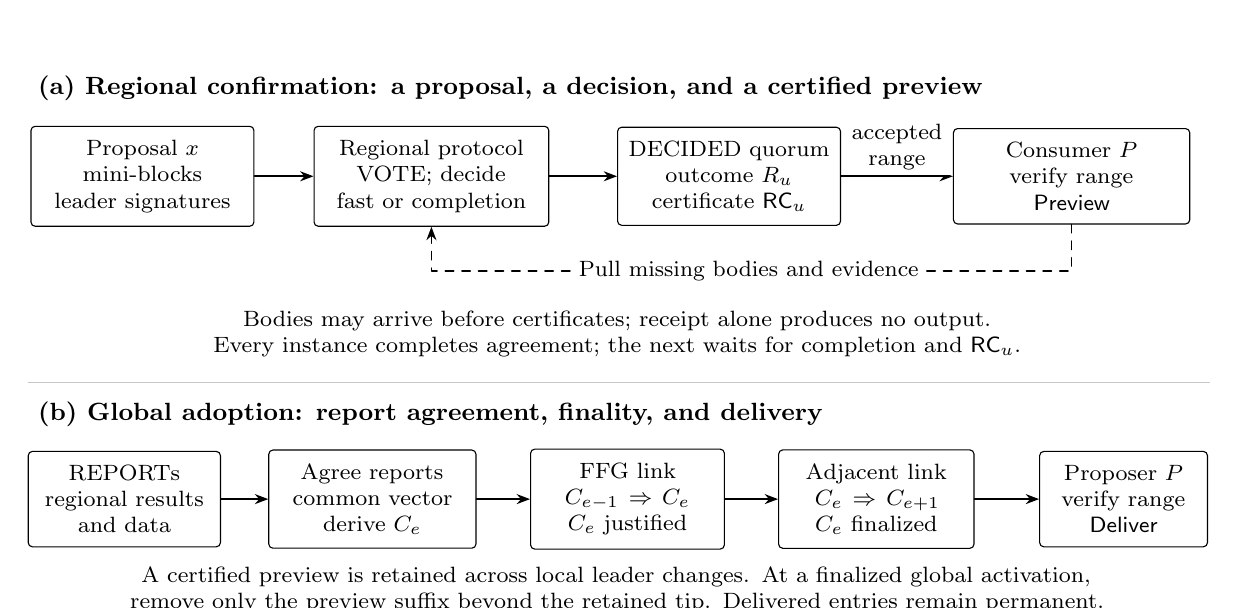
\begin{tikzpicture}[
  x=1cm,y=1cm,font=\small,line cap=round,line join=round,
  pipebox/.style={draw,rounded corners=1.5pt,fill=white,align=center,
    inner xsep=4pt,inner ysep=5pt,font=\footnotesize},
  pipeflow/.style={-{Stealth[length=1.7mm]},semithick},
  pipepull/.style={-{Stealth[length=1.7mm]},semithick,dashed},
  pipelabel/.style={font=\footnotesize,fill=white,inner sep=2pt,align=center}
]
  \node[anchor=west,font=\small\bfseries] at (0,7.70)
    {(a) Regional confirmation: a proposal, a decision, and a certified preview};
  \node[pipebox,text width=2.55cm,minimum height=1.18cm] (proposal) at (1.45,6.58)
    {Proposal $x$\\mini-blocks\\leader signatures};
  \node[pipebox,text width=2.70cm,minimum height=1.18cm] (decision) at (5.12,6.58)
    {Regional protocol\\VOTE; decide\\fast or completion};
  \node[pipebox,text width=2.55cm,minimum height=1.18cm] (certificate) at (8.90,6.58)
    {DECIDED quorum\\outcome $R_u$\\certificate $\RC_u$};
  \node[pipebox,text width=2.72cm,minimum height=1.18cm] (preview) at (13.25,6.58)
    {Consumer $P$\\verify range\\$\Tag{Preview}$};
  \draw[pipeflow] (proposal.east) -- (decision.west);
  \draw[pipeflow] (decision.east) -- (certificate.west);
  \draw[pipeflow] (certificate.east) -- node[pipelabel,above,text width=1.25cm]
    {accepted\\range} (preview.west);
  \draw[pipepull] (preview.south) -- (13.25,5.38) -- (5.12,5.38) -- (decision.south);
  \node[pipelabel] at (9.15,5.38) {Pull missing bodies and evidence};
  \node[pipelabel,text width=14.60cm] at (7.45,4.58)
    {Bodies may arrive before certificates; receipt alone produces no output.\\
     Every instance completes agreement; the next waits for completion and $\RC_u$.};

  \draw[gray!45] (0,3.96) -- (15.00,3.96);
  \node[anchor=west,font=\small\bfseries] at (0,3.56)
    {(b) Global adoption: report agreement, finality, and delivery};
  \node[pipebox,text width=2.16cm,minimum height=1.12cm] (reports) at (1.22,2.48)
    {REPORTs\\regional results\\and data};
  \node[pipebox,text width=2.35cm,minimum height=1.12cm] (agreement) at (4.37,2.48)
    {Agree reports\\common vector\\derive $C_e$};
  \node[pipebox,text width=2.18cm,minimum height=1.12cm] (justified) at (7.61,2.48)
    {FFG link\\$C_{e-1}\Rightarrow C_e$\\$C_e$ justified};
  \node[pipebox,text width=2.20cm,minimum height=1.12cm] (finalized) at (10.77,2.48)
    {Adjacent link\\$C_e\Rightarrow C_{e+1}$\\$C_e$ finalized};
  \node[pipebox,text width=1.85cm,minimum height=1.12cm] (deliver) at (13.91,2.48)
    {Proposer $P$\\verify range\\$\Tag{Deliver}$};
  \draw[pipeflow] (reports.east) -- (agreement.west);
  \draw[pipeflow] (agreement.east) -- (justified.west);
  \draw[pipeflow] (justified.east) -- (finalized.west);
  \draw[pipeflow] (finalized.east) -- (deliver.west);
  \node[pipelabel,text width=14.60cm] at (7.45,1.33)
    {A certified preview is retained across local leader changes. At a finalized global activation,\\
     remove only the preview suffix beyond the retained tip. Delivered entries remain permanent.};
\end{tikzpicture}

\caption{A mini-block stream's construction and delivery. Push is the primary
consumer path; pull repairs a missing object. Regional Preview and global
Deliver are different events. Arrows show dependencies, not equal-duration
rounds; the next regional instance waits for completion and its predecessor
certificate. No consumer execution or publication is
part of this pipeline.}
\label{fig:stream}
\end{figure}

\begin{example}[A missing middle mini-block]
The consumer has 100 and receives 101 and 103 but not 102. It asks a regional
holder for 102 and any missing range certificate. A response with a different
body fails the committed digest check; a correct response restores the chain
101--102--103. The receiver then outputs the eligible contiguous range once.
Receiving 103 first never permits skipping position 102.
\end{example}

\Needspace{22\baselineskip}
\subsection{Regional view changes}\label{sec:localchange}
Let the local cyclic schedule have cursor $j$, initially fixed by the activation.
The local view $\lv$ counts changes of that cursor. Planned changes occur at
instance numbers divisible by $N_R$; $K_R$ consecutive failed instances trigger
early replacement.

\begin{protocol}{alg:localchange}{Deterministic regional outcome transition}
\textbf{Input:} certified $R_{u-1}$ with view $\lv$, leader-list cursor $j$,
failure streak $z_{\mathrm R}$, and decision $x$ or $\botv$ for $I$.
\begin{enumerate}[label=\textbf{L\arabic*.}]
\item If the decision is $x\neq\botv$, adopt $x$'s end tip and put
$z_{\mathrm R}'=0$. Otherwise retain the tip and put
$z_{\mathrm R}'=z_{\mathrm R}+1$.
\item Let $\mathsf{planned}$ mean $u\equiv0\pmod{N_R}$ and
$\mathsf{failed}$ mean $z_{\mathrm R}'\geq K_R$.
If either holds, advance $j$ by one modulo $n_i$, increment $\lv$, and reset
$z_{\mathrm R}'=0$. If both hold, advance once. Otherwise retain $j,\lv$.
\item Form $R_u$ with this tip, next view and leader, and failure streak;
set $d_u=\Hash(x)$ for an accepted proposal and $d_u=\botv$ otherwise.
The successor becomes producer at instance $u+1$'s scheduled start, after
completion and predecessor-certificate availability. It starts at $R_u$'s tip.
\end{enumerate}
\end{protocol}

All responsive honest local members already hold each decided proposal. An individual
leader crash therefore needs no new whole-history transfer in a live region.
A recovering member restores its own persistent signing history and pulls the
missing certified public state needed to join a future scheduled instance;
it does not backfill votes for expired
instances. If an interrupted instance cannot acquire its outcome certificate,
the region cannot resume that global view merely by restoring connectivity.
The global protocol below can activate a fresh global view in another region
or, when no other region is ready, in the recovered current region. Neither
path waits for the failed instance or clears its persistent signing history.

\subsection{Backbone synchronization and global report agreement}\label{sec:global}
Global epoch $e$ occupies $[(e-1)T_G,eT_G)$. Its control participants are all of
$V$, independent of the active production region. Logical signed control
messages use the backbone; complete bodies are pushed on the primary path or
pulled and cached as in \cref{alg:pull}. An honest recipient of a validated
report serves its body thereafter. The synchronized protocol consumes a message
only when this complete object is available.

\begin{protocol}{alg:global}{A complete global epoch}
\textbf{Common initial state:} $C_{e-1}$, its justification proof, the adopted
stream and any older finality proofs. $C_0$ is justified and finalized.
\begin{enumerate}[label=\textbf{G\arabic*.}]
\item \textbf{At epoch start.} If the parent has a pending rotation already
finalized by an earlier link, verify that proof and apply its activation once.
Each member snapshots the earliest contiguous known extension from the resulting
cursor that fits the configured bounds, taking the longest such prefix and
never truncating a certified batch. An honest member sets READY true exactly
when it holds the complete verified parent prefix and evidence and is ready
to start the next global view from that prefix in its configured region;
otherwise it sets false and
continues pulling the missing state. A healthy eligible member with these data
must set true. It signs one report; READY binds the parent's exact tip and
the next global view after any pre-transition activation. No extension is required.
\item \textbf{Report agreement.} Run $N$ parallel instances of
\cref{alg:ab}, with domain $(\Tag{REPORT},c,e,g_{e-1})$, round length $\Delta_G$
and validity predicate $\Proc{ValidReport}$. After $N\Delta_G$, replace every
missing or equivocated origin by $\botv$ to obtain $\mathbf r_e$.
No global target is selected before this completion.
\item \textbf{Derive the target.} Apply \cref{alg:gtransition} to the common
parent, activation proof and report vector. Construct exactly $C_e$ in
\eqref{eq:global}. Retain its complete adopted prefix and transition evidence.
\item \textbf{FFG vote.} At elapsed time $N\Delta_G$, each eligible member
signs $(\Tag{FFG},c,e-1,g_{e-1},e,g_e)$ after the checks in
\cref{alg:finality}. Disseminate the vote through the backbone.
\item \textbf{Certificate.} By $(N+1)\Delta_G$, responsive honest members
have a quorum of votes. They form and disseminate the link certificate.
By $(N+2)\Delta_G$, process justification and finality. Push or announce the
new checkpoint and proof to consumers; missing data remains retrievable.
\item \textbf{Boundary.} Set $T_G\geq(N+3)\Delta_G$; the remaining margin
makes the certificates and newly activated regional initialization available
before the next common boundary. Carry the adopted state to epoch $e+1$.
\end{enumerate}
\end{protocol}

Report agreement is an explicit, deliberately conservative convergence mechanism.
It already selects a unique control chain under synchrony. FFG supplies the
chosen two-link finality and activation rule on that chain; it is not invoked
as an unexplained solution to inconsistent reports. This construction pays for
report agreement even during a good epoch. Its performance bounds are derived
for this protocol and do not inherit Ethereum's performance claims.

A planned global view change becomes due $N_G$ checkpoint epochs after
activation; $K_G$ consecutive no-progress epochs trigger recovery.

\begin{protocol}{alg:gtransition}{Global state transition and region selection}
\textbf{Input:} common parent state, any finality-based activation applied at
epoch start, and $\mathbf r_e$. Fields not explicitly updated retain their
effective-state values.
\begin{enumerate}[label=\textbf{T\arabic*.}]
\item \textbf{Pending, not activated.} If a rotation remains pending, output
$\Tag{CONFIRM}$ with exactly the same stream tip, region and pending package.
No new regional data is adopted; increment $z_{\mathrm G}$ by one.
\item \textbf{Available extension.} Otherwise, among valid reported regional
chains rooted at the effective cursor, choose the longest one; break an exact
equality by its semantic digest. Let its endpoint be $(R^+,h^+,q^+)$, or retain
the effective-state cursor and tip if no extension exists. These chains are compatible by
\cref{lem:rcunique}. Put $z_{\mathrm G}^+=0$ if $h^+>h$, and $z_{\mathrm G}^+=z_{\mathrm G}+1$ otherwise.
\item \textbf{Eligible successor.} A region $j$ is ready if true READY
reports for the parent's exact tip have total weight $>2W_j/3$.
A change is due if $e-e_{\gv}\geq N_G$ or $z_{\mathrm G}^+\geq K_G$.
If due and a different region is ready, choose the first such region after $i$
in the configured cyclic list. Otherwise, if $z_{\mathrm G}^+\geq K_G$, no different region
is ready and $i$ is ready, choose $j=i$ for recovery. If a region is selected,
output $\Tag{ROTATE}$, retain the parent's data tip and the effective-state
regional cursor, and store
\[
 p=(\gv+1,j,\ell_0',h,q,R,e,\mathsf{readyRefs},\mathsf{reason}).
\]
Here $\ell_0'$ is that region's configured first leader; readyRefs and reason
are the deterministic fields defined in \cref{sec:gobjects}. Increment
$z_{\mathrm G}$ by one because the retained data tip does not grow. ROTATE does not
simultaneously adopt a new range: its readiness proof refers to the retained tip.
The proposed regional extension remains a preview. Selection of $j=i$ uses
the same finality and activation rules, with a fresh global view $\gv+1$ and $R_0$;
it does not reuse old instance identifiers or erase signing history.
\item \textbf{No rotation.} Otherwise adopt $(R^+,h^+,q^+)$, set the failure
count to $z_{\mathrm G}^+$, and output ADVANCE if the data tip grows or HOLD otherwise.
If no region is selected, service can continue in the current global view.
\end{enumerate}
\end{protocol}

A global report may advance the regional cursor through certified gaps without
advancing the data tip. These cursor updates are retained and consume report
capacity. An honest reporter takes the earliest contiguous extension that fits
the bounds; it never drops an intervening outcome or truncates a certified batch.
Global no-progress means no new adopted mini-block, not low transaction volume
or dissatisfaction with a producer's ordering policy.

\Needspace{30\baselineskip}
\subsection{Finality, activation and consumer verification}\label{sec:finality}
\begin{protocol}{alg:finality}{FFG links and geographic activation}
\textbf{Persistent state:} signed FFG history; justified and finalized checkpoints.
\begin{enumerate}[label=\textbf{F\arabic*.}]
\item \textbf{Before voting.} Verify the target derived by \cref{alg:global},
its complete adopted data and its parent justification. Sign at most one
statement for a target epoch. Never sign a pair with source/target epochs
$s_1<s_2<t_2<t_1$, nor a target conflicting with the known finalized prefix.
The concrete epoch protocol uses only $(e-1,e)$ links.
\item \textbf{Verify a link.} A link $C_s\Rightarrow C_t$ contains
$\QC_V(\Tag{FFG},c,s,g_s,t,g_t)$, the identified checkpoints and a path of
valid checkpoint transitions from $C_s$ to $C_t$. Require $s<t$, exact matching
hashes and a justified source.
A valid link justifies its target.
\item \textbf{Finalize.} A justified $C_e$ is finalized by a link to its direct
child $C_{e+1}$. Ancestors are finalized too. An independently verifiable proof
contains the justification chain back to an already trusted anchor and this
adjacent link. Equal stream roots at different epochs do not mean equal
checkpoint identities.
\item \textbf{Activate.} If a pending ROTATE $C_r$ is finalized by the link
$C_r\Rightarrow C_{r+1}$, its successor starts at the fixed boundary beginning
epoch $r+2$, namely time $(r+1)T_G$. Before that boundary it verifies the finality
proof and retained data. The proof fixes $R_0$, global view, region and initial
leader for the new service. A node missing these objects does not start.
\item \textbf{Represent activation.} At the start of epoch $r+2$, apply this
proof to the strict ancestor ROTATE: set $(\gv,i,\ell_0)$ to its named successor,
$v_{\mathrm L,0}=0$, $A=g_r$, $R=R_0$, $z_{\mathrm G}=0$, $e_{\gv}=r+2$, and $p=\varnothing$;
preserve $(h,q)$. The first subsequent global target records this pre-transition
before evaluating \cref{alg:gtransition}. Checkpoints $C_r$ and
$C_{r+1}$ remain unchanged. New regional data cites the activation proof.
\end{enumerate}
\end{protocol}

At the activation boundary, every responsive honest global member has a valid
proof of the same activation and full retained data under the epoch budget. A healthy selected
region therefore starts from one common $R_0$, including after recovery in the
same region. An unavailable chosen region
cannot begin service; global epochs still run, detect the continued lack of
progress and attempt a later successor. A READY quorum proves possession at
its signing point, not immunity from a subsequent regional outage.

An old region disconnected from the control plane can continue to show signed
previews to stale clients. It cannot extend the accepted global history after
its replacement. All newly adopted data must match the effective global view
of the common global state. Consumers learn replacement from a finality proof,
not from an unauthenticated redirect or a private timeout.

\begin{example}[Local failure and geographic failure]
Suppose regional certificate $\RC_u$ covers position 110. If its leader stops,
$K_R$ consecutive completed bottom instances replace it locally; the successor
extends 110. Now suppose the whole region becomes unreachable while the global
adopted tip is 100 and 101--110 exists only as regional preview. After $K_G$
no-progress epochs, a ready region can be named by ROTATE at $C_r$. CONFIRM at
$C_{r+1}$ finalizes that record, and the new region starts at epoch $r+2$ from
100. The consumer keeps every delivered position and drops only the unretained
preview. Had the global chain already adopted 110, the handoff would have to
retain 110, even if its checkpoint had not yet finalized when the outage began.
\end{example}

\Needspace{20\baselineskip}
\subsection{Equivocation and invalid inputs}\label{sec:evidence}
\begin{protocol}{alg:evidence}{Transferable conflict evidence}
\textbf{Input:} two signed statements $(S,m,\sigma)$ and $(S,m',\sigma')$.
\begin{enumerate}[label=\textbf{E\arabic*.}]
\item Verify both signatures and the configured identity, chain and message
domain. Reject unless both are well-formed statements of the compared type.
\item Return evidence if one of the following exact predicates holds:
\begin{enumerate}[label=\textnormal{(\alph*)}]
\item ORDER: equal $(c,\gv,u,h)$ but different mini-block header digests;
\item PROPOSE or VOTE: equal instance $I$ but different proposal digests;
\item DECIDED: equal $I$ but different outcome digests, including different parents;
\item REPORT: equal $(c,e,g_{e-1},S)$ but different semantic reports;
\item FFG: the same target epoch with different source/target statements, or
$s_1<s_2<t_2<t_1$ (in either ordering of the pair).
\end{enumerate}
\item Store valid evidence. Propagate at most one pair per signer, statement
type and comparison key (instance, report domain or target-epoch pair), as a bounded
control object. Retain
signing weights for the fixed configuration; evidence does not change quorum
thresholds mid-instance.
\end{enumerate}
\end{protocol}

Verify and extract evidence before discarding a conflicting authenticated
statement from ordinary processing. Duplicate encodings of one semantic
statement are not an offense. Relaying two origin values in \cref{alg:ab} is
required recovery behavior and is not a double vote by the relay. Silence,
a missing DATA response and legitimate view changes are not equivocation. Penalty amounts and adjudication mechanisms are outside
the service.

\section{Correctness and Soundness}\label{sec:proofs}
All results concern the fixed configuration and fault/delivery envelope in
Section~\ref{sec:model}. Cryptographic failures contribute a negligible error;
the remaining arguments are deterministic.

\begin{lemma}[Quorum intersection]\label[lemma]{lem:intersection}
Two quorums of a committee of weight $W_Q$ intersect in weight greater than
$W_Q/3$. Under a Byzantine bound below $W_Q/3$, they share an honest signer.
\end{lemma}
\begin{proof}
For signer sets $U,U'$, $\wt(U\cap U')\geq\wt(U)+\wt(U')-W_Q>W_Q/3$.
For an intersection with responsive honest members, use the bound on the union
of Byzantine and potentially unavailable members.
\end{proof}

\begin{lemma}[Authenticated origin broadcast]\label[lemma]{lem:ab}
In \cref{alg:ab}, all responsive honest members return the same value or bottom.
If the origin is honest and responsive, they return its valid input. Every
non-bottom output has a valid witness. The protocol terminates in $n$ rounds,
where $n$ is the committee size, if at least one member is honest and responsive
and complete-object delivery respects the round bound.
\end{lemma}
\begin{proof}
Consider a value retained by an honest responsive member in round $r$. If its
chain contains an honest responsive signer at position $k$, that signer sent
the length-$k$ prefix to all responsive members in round $k$. Every such member
receives it by that deadline and either retains it or already has two values.
If the chain has no honest responsive signer, its length is at most $n-1$.
The retaining member extends and forwards it for round $r+1$, unless it already
forwarded that value, in which case its earlier send suffices. A length-$n$
chain necessarily contains an honest responsive signer. Thus every value
retained honestly is, by round $n$, retained by every honest responsive member
or meets a receiver that already has two values.

If any honest responsive member has two values, apply this fact to both:
all such members end with two values and return bottom. Otherwise a nonempty
honest set propagates its sole value to all others, so all return it. If all
sets are empty, all return bottom. An honest origin signs only its own input;
unforgeability and first-round delivery exclude a second value or empty set.
Every retained value passed the fixed validity predicate, and fixed deadlines
ensure termination. The proof needs agreement on singleton-versus-multiple
outputs; cap-two sets need not contain the same pair when an origin sends three
or more different values.
\end{proof}

\begin{lemma}[Weighted completion]\label[lemma]{lem:ba}
In a live regional instance, \cref{alg:ba} has agreement, termination,
unanimity validity and external validity, with duration $n_i\Delta_R$.
\end{lemma}
\begin{proof}
\Cref{lem:ab} gives the same origin-output vector to all responsive honest
members. At most one value can have vector support $>2W_i/3$. If all responsive
honest inputs equal $x$, honest-origin validity gives $x$ that much support.
If all such inputs are bottom, non-bottom support is confined to weight below
$W_i/3$, so the output is bottom. A returned non-bottom value has the checked
proposal and vote certificate. The parallel broadcasts take $n_i$ rounds.
\end{proof}

\begin{theorem}[Regional broadcast]\label[theorem]{thm:bb}
During a live regional instance, all responsive honest members decide the same
valid proposal or bottom. An honest responsive leader's eligible proposal is
decided. Its internal good-case latency is at most $2\delta_R$ when actual
complete-object delay is at most $\delta_R$.
\end{theorem}
\begin{proof}
Two distinct VOTE quorums would share an honest signer, contradicting one vote
per instance. Thus there is at most one non-bottom lock value $x$. If an honest
member fast decides by $2\Delta_R$, it forwards the complete certificate;
all responsive honest members receive it by $3\Delta_R$, before snapshotting.
Their completion inputs are all $x$, so \cref{lem:ba} preserves the decision.
If no honest member fast decides, completion agreement determines their common
output. These cases cover two fast decisions, a fast decision followed by
completion, and completion-only decisions. All non-bottom outputs satisfy the
proposal-validity predicate.

An honest leader sends the same valid proposal to all responsive honest
members. Their votes alone exceed the threshold. Proposal delivery and vote
delivery take two actual delays, within the fast cutoff. Certificate export
and completion remain separate later obligations.
\end{proof}

\begin{lemma}[Unique exported regional chain]\label[lemma]{lem:rcunique}
Within one global view at most one outcome per instance has a valid $\RC_u$.
Certified outcomes form one chain from the authorized $R_0$, and each certified
non-bottom range satisfies the producer and content rules. These claims do not
require a failed region to finish its internal broadcast.
\end{lemma}
\begin{proof}
Two DECIDED quorums for one $I$ would share an honest member that signed two
outcome hashes. The hash binds the parent, so induction from $R_0$ gives one
certified chain. Honest members verify the predecessor's authorization evidence before entering
the next instance and compute the prescribed transition. A certificate contains
an honest signer that verified every non-bottom body and its producer authority.
Loss of synchrony can prevent completion or invalidate the internal fast-agreement
argument; it cannot produce two exported quorums under these persistent
sign-once and Byzantine-weight assumptions.
\end{proof}

\begin{theorem}[Global agreement and authority]\label[theorem]{thm:global}
Under the global envelope, all responsive honest members derive the same $C_e$
in every epoch, justify it and finalize $C_{e-1}$. Adopted data prefixes are
monotone. A finalized ROTATE authorizes its unique named successor at the
specified boundary and preserves all previously globally adopted data.
\end{theorem}
\begin{proof}
Induct from genesis. The previous certificate phase makes the parent,
justification and required activation statement common before the epoch begins.
The report-validity predicate is consequently common. \Cref{lem:ab} supplies
the same report vector. The transition is deterministic; by
\cref{lem:rcunique}, its eligible regional extensions are compatible. Every
responsive honest member therefore derives the same target and retains its
complete adopted data.

Their weight exceeds $2W/3$, so their FFG votes establish the parent-to-child
link in one $\Delta_G$, and certificate dissemination finishes in another.
Both source and target epochs increase, satisfying honest signing constraints.
The target is justified and its parent finalized. ADVANCE extends the data
prefix; HOLD and CONFIRM retain it; ROTATE retains its parent's prefix and stores
one pending successor. Activation consumes the finality proof of that strict
ancestor and cannot mutate an existing checkpoint. This also holds when the
region is unchanged: the new global view separates all regional signing domains,
and its $R_0$ inherits the same retained global tip. Induction gives monotone
prefixes and a unique authorization chain. A conflicting certified target at
one epoch would also require an honest FFG double vote by quorum intersection.
\end{proof}
The FFG vocabulary follows Casper~\cite{ffg}. This proof establishes it on our
explicit synchronous control chain; it does not assume that FFG alone makes
inconsistent reports converge.

\begin{theorem}[Verification soundness and stream safety]\label[theorem]{thm:sound}
\Cref{alg:pull} satisfies the validity, integrity, agreement and verification
clauses of \cref{def:service}. Regional previews are prefix-compatible across
local changes. A global view change cannot remove a delivered entry.
\end{theorem}
\begin{proof}
An ORDER signature binds the producer to the header, and hash binding fixes
its ordered body and predecessor. \Cref{lem:rcunique} supplies one certified
regional chain with deterministic local authorization changes.
\Cref{thm:global} supplies one global chain with monotone adopted prefixes and
unique geographic transitions. Finalized checkpoints lie on that chain.
Consumers verify these objects and append only complete, contiguous, previously
undelivered positions. Thus their delivered logs are prefixes of one sequence
and grow monotonically.

Changing contents or their order breaks a commitment; changing the parent,
position, view or global view changes a signed header. A substituted producer
requires either a valid authorization for that position or a forged signature.
A substituted confirmed history requires conflicting regional or global
certificates, excluded above. Serving the same object through a different peer
supplies none of these missing proofs. Correct complete evidence passes the
specified checks. At handoff, the retained tip includes every prior globally
adopted entry, hence every delivered entry. Applying every intervening activation
in order truncates an old preview at its first discarded suffix, even if a later
global view reuses those positions. Only an unretained preview is removed.
\end{proof}

\begin{lemma}[Data retention and repair]\label[lemma]{lem:pull}
A globally justified checkpoint has responsive honest holders of its complete
adopted prefix. For a bounded requested object, if $a$ attempted suppliers fail
before a responsive honest holder, retrieval takes at most $(a+1)\theta$ after
the first request, where $\theta$ is the complete attempt deadline. Regional
preview repair has the analogous bound during a live regional interval.
\end{lemma}
\begin{proof}
Responsive honest global members have weight $>2W/3$, possess the common adopted
prefix and retain it before voting. A verified vote quorum also intersects this
responsive set. Thus its data cannot exist solely at unavailable holders.
Each unsuccessful attempt costs at most $\theta$; an honest holder returns the
complete original object within that deadline. Its verification is independent
of the supplier being the producer. The local claim uses the responsive holders
after regional dissemination. Multiple chunks incur the sum of their bounds.
\end{proof}

\begin{theorem}[Service liveness]\label[theorem]{thm:live}
Assume the global envelope, a healthy eligible region that remains available,
and the capacity and minimum-tenure conditions in
\cref{sec:latency}. A finite sequence of failed local leaders is bypassed.
Following a regional outage and finitely many unproductive successor regions,
a healthy successor, possibly the recovered current region, resumes confirmation
and global delivery. During continuing
healthy service, live consumers' delivered logs grow without bound.
\end{theorem}
\begin{proof}
Each live regional instance completes within its scheduled spacing by
\cref{thm:bb,lem:ba}. A bottom outcome increments the shared counter;
$K_R$ such outcomes move to the next leader, possibly earlier at a planned
boundary. Within at most $n_i$ tenures an honest responsive leader is reached.
Its eligible batch is confirmed, even if its transaction lists are empty.

If global progress stops, the common counter reaches $K_G$. Responsive members
of a healthy eligible region retain the global prefix and originate true READY
reports, even if an old regional instance has no outcome certificate. Their
weight gives a ready quorum. Report agreement delivers these reports without
completion of the failed instance. Distinct-region selections advance along
the cyclic list and cannot skip a continuously ready healthy region. If no
different region is ready, a ready current region is selected for recovery.
Thus after finitely many unsuccessful selections a healthy region is activated.
ROTATE and its confirming child finalize its authorization, and the clock fixes
the common start from a fresh $R_0$. The failed global view's decisions cannot
block these new instances. The minimum-tenure
condition allows a healthy successor to finish local recovery and report a new
batch before geographic guards replace it again.

Pull and report propagation supply that batch's data. The configured report
budget admits contiguous extensions and drains a bounded backlog. Subsequent
FFG links finalize adopted data; \cref{lem:pull} delivers it to live consumers.
Repeating this argument gives unbounded growth. It requires neither cooperation
from the failed region nor inclusion of a particular client transaction.
\end{proof}

\begin{proposition}[Sound equivocation evidence]\label[proposition]{prop:evidence}
Every accepted evidence pair in \cref{alg:evidence} identifies incompatible
statements signed by the named member. An honest member following the relevant
signing rules cannot produce such a pair.
\end{proposition}
\begin{proof}
Both signatures authenticate the exact comparison domain. Each listed predicate
violates its sign-once rule or the FFG surround rule. Different permitted instances,
views, configurations or relayed origin values do not by themselves satisfy
these predicates. Unforgeability excludes attributing an unsigned statement to
an honest member. This proves attribution of conflicting statements, not fault
attribution for an unanswered request or the size of a financial penalty.
\end{proof}

\section{Latency, Communication and Synchronization}\label{sec:complexity}
\subsection{Timing and capacity}\label{sec:latency}
For one complete bounded range, let
\begin{equation}\label{eq:pullbound}
 F_R=(a_R+1)\theta_R,\qquad F_G=(a_G+1)\theta_G,
\end{equation}
where $a_R,a_G$ count failed attempts before a usable holder. A useful announced
tip is discovered within $A_R=T_A+\Delta_R$ regionally and
$A_G=T_A+\Delta_G$ globally. For a consumer path use $A_P=T_A+\Delta_P$,
where $\Delta_P$ includes its announcement propagation. For $J$ sequential
chunks, use $\sum_{j=1}^J(a_j+1)\theta_j$. Let $S_G$ denote this bound for all
missing handoff state and $F_P$ the corresponding consumer repair bound.

Let $Q$ bound the report epochs needed to adopt a retrievable regional outcome
and all its still-unadopted predecessors while the global view stays active,
after an honest participating reporter holds those complete objects.
This is a workload bound, not a consequence of the maximum packing limits.
In a live epoch, an honest reporter includes the longest fitting contiguous
prefix, so at least one complete pending outcome can be adopted. If there are
at most $J_0$ pending outcomes up to a target when that reporter holds them,
$Q\leq J_0$ suffices: later outcomes are appended behind that target and cannot
overtake it. These are adoption epochs executing ADVANCE/HOLD, not epochs
spent on pending ROTATE/CONFIRM. Let $F_{\rm sync}$ be the sum of the per-chunk
global pull bounds for obtaining those objects; it equals $F_G$ for one bounded
request and is larger when several sequential requests are required.
A configured arrival envelope and adequate sustained byte service
can give a uniform $J_0$; otherwise use the actual backlog for that target.
The limits $b_G,B_G$ must permit each individual outcome and its relative
evidence in full. Nominal rates $b_G/T_G,B_G/T_G$ are only packing upper bounds;
they do not establish a service rate when outcomes have variable sizes.
For $n_{\max}=\max_i n_i$ and $\tau_{\max}=\max_i\tau_R(i)$, define
\[
 L_{\rm sync}=A_G+F_{\rm sync}+QT_G,\qquad
 L_{\rm start}=(n_{\max}N_R+1)\tau_{\max}.
\]
To prevent repeatedly replacing a healthy newly activated region before it can
produce a reportable batch, require
\begin{equation}\label{eq:tenure}
 \min\{K_G,N_G\}T_G>L_{\rm start}+L_{\rm sync}+2T_G.
\end{equation}
The extra epochs cover report-cutoff alignment and the adopting epoch. This is
a conservative sufficient condition, not an optimal timer setting.

\subsection{Normal service and missing-data cases}
With accumulation time $L_{\rm build}$ and wait $L_{\rm wait}<\tau_R$ to the
next regional instance, the good-case bounds are
\begin{align}
 L_{\rm regional}&\leq2\delta_R,\label{eq:fast}\\
 L_{\rm preview}&\leq L_{\rm build}+L_{\rm wait}+4\delta_R+\delta_P.
 \label{eq:preview}
\end{align}
Two delays decide internally; one gathers DECIDED signatures and one
conservatively disseminates the exported certificate. $\delta_P$ covers the
complete-object consumer path. The next serialized instance still waits at
least $(n_i+5)\Delta_R$. Hash announcement followed by retrieval does not by
itself meet the complete-object premise of the $2\delta_R$ bound.

After regional certification, a conservative finalized-delivery bound in a
continuing healthy global view is
\begin{equation}\label{eq:deliver}
 L_{\rm final}\leq A_G+F_{\rm sync}+(Q+3)T_G+A_P+F_P.
\end{equation}
Besides backlog, this budgets one report-alignment epoch, one adopting epoch
and its confirming successor. An unadopted preview cancelled at a handoff has
no finalized-delivery promise. Regional throughput is at most $b_R/\tau_R$;
end-to-end delivery is also limited by global outcome and byte budgets.

\begin{table}[htbp]\centering\small
\begin{tabularx}{\textwidth}{@{}p{.33\textwidth}Y@{}}\toprule
Delivery case & Additional cost after data exists\\\midrule
Primary push succeeds & Primary data/certificate path; no consumer pull.\\
Known gap, first supplier honest & At most $\theta_R$ or $\theta_G$.\\
$a$ suppliers fail first & At most $(a+1)\theta$ for one bounded range.\\
Gap discovered by periodic announcement & Add the relevant $A_R,A_G$ or $A_P$.\\
$J$ missing chunks & Sum their attempt and verification bounds.\\
No retained reachable copy & No finite retrieval or lossless-recovery bound.\\\bottomrule
\end{tabularx}
\caption{Repair changes transport, not the confirmation predicate.}
\end{table}

\subsection{Local and geographic recovery}\label{sec:recoverybounds}
For $q$ continuously unproductive local leader tenures followed by an honest
leader in a live region,
a conservative failure-to-first-preview bound is
\begin{equation}\label{eq:localrecover}
 L_R(q)\leq(qK_R+1)\tau_R+4\delta_R+\delta_P.
\end{equation}
The extra spacing covers failure inside an outstanding instance. Planned
boundaries can shorten failed tenures. Add $A_P+F_R$ if the consumer repairs
the first result. A planned local handoff to an honest, synchronized successor
takes at most $4\delta_R+\delta_P$ after proposal construction at its declared
boundary. A recovering successor adds its state-transfer time before joining
an eligible future instance.
An intermittent Byzantine leader can reset the failure streak by producing a
valid batch. For a bound to the first \emph{honest successor} rather than any
resumed output, replace $qK_R$ in \eqref{eq:localrecover} by $qN_R$:
the next planned boundary occurs within $N_R$ instances of every tenure.
We use this more conservative class in $L_{\rm start}$. Actual stream progress
can occur earlier through a Byzantine leader's valid outputs.

For a geographic outage or an interrupted regional instance requiring a fresh
global view, let $L_{\rm tail}$ bound the time until the last
previously produced but unadopted old-region range advances the global tip.
Such late data resets the no-progress counter, so this term cannot be silently
omitted. Let $T_{\rm ready}$ cover successor synchronization and READY-report
alignment; for a cold successor, $T_{\rm ready}\leq S_G+T_G$ once its inputs are
available. If the next chosen region is healthy, a conservative bound is
\begin{equation}\label{eq:georecover}
\begin{split}
 L_G\leq{}&L_{\rm tail}+T_G+K_GT_G+T_{\rm ready}+2T_G\\
          &{}+L_R(q)+A_P+F_P.
\end{split}
\end{equation}
The terms cover detection alignment, the no-progress guard, readiness,
ROTATE/CONFIRM and the fixed activation boundary, and first successor preview.
Use the $N_R$ variant of $L_R(q)$ for intermittent Byzantine tenures.
Readiness and guard formation may overlap; the bound does not subtract that
overlap. To obtain a new finalized Deliver, add \eqref{eq:deliver} for the
successor range. For a planned geographic handoff measured from its due boundary,
omit $L_{\rm tail}+T_G+K_GT_G$, retaining any readiness wait and the finality
stages. Each unsuccessful selected region adds another such detection and
transition interval. No finite bound follows without a global quorum, usable
honest backbone paths, retained bytes, transfer capacity and an eventual healthy
eligible successor. Recovery in the same region uses this bound and the same
READY reports and ROTATE/CONFIRM epochs. It adds no message type, quorum or
round to normal service; it still pays the global recovery delay.

\subsection{Control communication and verification}\label{sec:controlcost}
Let $\kappa$ be signature-plus-signer bits; $L$ bound semantic metadata,
including certificate/history evidence but excluding a new signature chain
and bulk body; and $v$ bound underlying metadata signature checks.
Let $E_B$ be the number of directed backbone arcs used by dissemination.
The backbone bounds assume each logical multicast forwards its envelope at
most once per arc; payload transfer is counted separately below.
For $n$ parallel authenticated-broadcast origins, cap-two forwarding gives at
most $2n^2$ logical multicasts over the entire invocation, each of size at most
$L+n\kappa$. Thus the control-bit bounds are
\begin{align}
 C_{\rm direct}(n,L)&=O(n^3(L+n\kappa)),\label{eq:directcost}\\
 C_{\rm backbone}(n,L)&=O(E_Bn^2(L+n\kappa)).\label{eq:backbonecost}
\end{align}
The respective transmission counts are $O(n^3)$ direct messages and $O(E_Bn^2)$
backbone arc transmissions. Signature generation is $O(n^2)$. Straightforward
uncached endpoint verification costs $O(n^3(n+v))$ signature checks; verification
at each forwarding hop can add $O(E_Bn^2(n+v))$ checks.

\begin{table}[htbp]\centering\small
\begin{tabularx}{\textwidth}{@{}p{.30\textwidth}p{.19\textwidth}Y@{}}\toprule
Component & Transmissions & Control bits\\\midrule
Regional fast path and export & $O(n_i^2)$ & $O(n_i^2L_R^c+n_i^3\kappa)$\\
Mandatory regional completion & $O(n_i^3)$ & $O(n_i^3(L_R^c+n_i\kappa))$\\
Global report agreement & $O(E_BN^2)$ & $O(E_BN^2(L_G^c+N\kappa))$\\
FFG votes and certificate export & $O(E_BN)$ & $O(E_BNL_G^c+E_BN^2\kappa)$\\\bottomrule
\end{tabularx}
\caption{Reference costs without signature aggregation. $L_R^c,L_G^c$ are
bounded metadata sizes. Each local attempt pays both regional rows, including
on the good path; each geographic attempt pays its participating epoch costs.}
\end{table}

If evidence contains $\eta$ records of at most $\ell$ bits, use
$L=L_0+\eta\ell$; a short header does not make its recursive proof constant-size.
A consumer syncing from genesis pays for its required full history. The
completion is deliberately conservative: a stake bound alone does not imply
that at most one third of the \emph{identities} are Byzantine. Protocol-admitted
traffic is bounded; unlimited Byzantine wire flooding is outside these counts.
Over duration $T$, with $U$ new-certificate events, the conservative
all-holder policy adds $O(N\lceil T/T_A\rceil+NU)$ announcements; forwarding
multiplies backbone announcements by at most $E_B$. For $J$ bounded pull requests
and at most $a$ failures before success, requests/replies add $O((a+1)J)$ logical
messages, weighted by path lengths for physical-link counts. If $Z$ distinct
conflict proofs are forwarded, add $O(E_BZ)$ backbone transmissions and their
bounded proof sizes. Announcements, evidence and consumer subscriptions are
interval costs, not free per-instance operations.

\subsection{Payload and retained state}\label{sec:payloadcost}
Let $X$ be the distinct body bytes requested in an interval, including unconfirmed proposals
and unretained previews later discarded, and $M$ the sum of missing bytes over $R$ receivers.
Then $M\leq RX$; if one of the $R$ receivers already holds everything,
$M=(R-1)X$ when all others need the full range. A transfer plan sending each
needed content digest once per receiver uses $M$ body bytes. The primary path,
however, pushes per mini-block and may repeat identical bodies at different
positions. Define $M_0$ as the sum of all primary-push body sizes across their
destinations: normal loss-free service with no repair costs $M_0$ body bytes.
Let $M_r$ be the sum of still-missing
body sizes entering repair. With at most $a$ failed attempts per repaired body,
each response capped at its requested length,
\begin{equation}\label{eq:payload}
 B_{\rm body}\leq M_0+(a+1)M_r\leq(a+2)M.
\end{equation}
The last inequality assumes $M_0,M_r\leq M$, as when each receiver has at most
one primary push and one sequential repair campaign per initially missing body.
Pure pull with no primary push gives $(a+1)M$. A late primary push racing a
successful pull explains the extra copy; cancellation cannot retract in-flight
bytes. Body caching is shared across all origin-report wrappers, not just
across repetitions of the same report identifier.
Announcements, requests and certificates are additional control traffic.
Physical link-byte cost multiplies each transfer by its route length; it is
not the $E_B$ factor for a flooded compact control envelope.

The leader sends one primary full copy to $P$ while regional validators obtain
the proposal for voting. Global report verification can require every responsive
global member to fetch newly adopted bodies. Backbone/pull avoids copying full
bodies along every logical vote edge, but does not eliminate those required
replicas. If caching is disabled, conservative complete-object bounds are
$O(n_i^3(B_R+L_R^c+n_i\kappa))$ bits for local completion and
$O(E_BN^2(B_G+L_G^c+N\kappa))$ for global report exchange.

A full replica retains $O(8X_{\rm history}+A_{\rm history})$ bits, where $X$ is
body bytes and $A$ is evidence bits. Constant byte/bit conversions are suppressed
in the preceding asymptotic bounds. A cold handoff pays for
both missing data and missing evidence; a hot handoff may fetch only a new
authorization proof. No constant-size root reconstructs unavailable bytes.
Pruning requires a separately specified archive/retrieval rule; the reference
retains the configuration's history.

\subsection{Limits of the analyzed cases}
The bounds cover healthy service, consumer-path loss, failed local leaders,
planned switches, whole-region outages, unavailable successors and cold state
transfer. If a required synchronization bound fails during authenticated
broadcast, its agreement proof is unavailable. If responsive global weight is
insufficient, finality and geographic activation may stop. An unavailable
required payload or unbounded backlog has no finite recovery bound. These are
explicit boundaries of the service envelope, not additional constant-latency
cases. Execution and publication by a consumer remain outside every bound.

\section*{Relation to Existing Specifications}
Mathematical records, predicates and state transitions follow the presentation
style of the Ethereum Yellow Paper~\cite{yellowpaper}. The model--task--algorithm--proof
organization follows the corrected optimistic reliable-broadcast paper~\cite{optimistic}.
Our regional primitive is signed and synchronous, not that paper's signature-free
asynchronous RBC. Its fast rule follows $2\delta$-BB~\cite{goodcase}; weighted
completion and global report agreement are instantiated here. Signed-chain
broadcast follows Dolev and Strong~\cite{ds}. The citations identify origins;
the necessary algorithms and composition proofs are included in this paper.

\appendix
\section{Complete Authenticated Broadcast}\label{app:ab}
Fix a committee $Q$ of $n$ identities, origin $o\in Q$, common instance domain
$J$, deterministic complete-object validity predicate $F_J$, and round length
$\Delta$. The special input value $\botv$ has an empty witness. Invalid or absent
traffic is not a signed bottom input, although the algorithm's bottom output
can represent an absent, ambiguous or genuinely bottom-valued origin. The
calling protocols intentionally treat these outputs identically.

For semantic value $z$, a length-$r$ chain is
\[
 C_r=((p_1,\sigma_1),\ldots,(p_r,\sigma_r)),\quad p_1=o,
\]
\[
 \sigma_k=\Sig_{p_k}(\Tag{CHAIN},J,o,z,k,C_{k-1}),\qquad C_0=().
\]
$\Proc{ChainValid}$ checks $1\leq r\leq n$, distinct configured identities,
first signer $o$, and each nested signature. The detached witness $\omega_z$
must satisfy $F_J(z,\omega_z)$. Different valid witnesses are not different
semantic values. Receivers obtain the complete required body before accepting;
honest forwarding members become servers for it.

\begin{protocol}{alg:ab}{Signed synchronous broadcast of one origin's value}
\textbf{State at $p\in Q$:} retained set $A_p=\varnothing$, of at most two
semantic values; forwarded set $F_p=\varnothing$. Round $r$ has send boundary
$(r-1)\Delta$ and receive deadline $r\Delta$; there are $n$ rounds.
\begin{enumerate}[label=\textbf{A\arabic*.}]
\item \textbf{Origin at round 1.} For valid input $z$, send
$(J,o,z,C_1,\omega_z)$ to all members, including itself. Mark $z$ forwarded
at the origin. Self-delivery is immediate.
\item \textbf{Receive.} Verify the chain and complete witness. Associate a
length-$r$ chain only with round $r$; buffer early arrivals and ignore an object
not completely valid by $r\Delta$. Enforce configured limits and admission
quotas while reserving every prescribed honest message.
\item \textbf{At deadline $r\Delta$.} Process valid length-$r$ packets in
semantic-digest order. Retain $z$ and its witness if already retained or if
$|A_p|<2$; ignore other values for this call. If $r<n$, $z$ is retained but not
forwarded, and some received valid chain for $z$ omits $p$, append $p$'s signature
and multicast the length-$(r+1)$ chain at this boundary. Mark it forwarded.
Forward at most once per retained value per origin over the whole invocation.
Continue prescribed forwarding after retaining two values.
\item \textbf{At deadline $n\Delta$.} After processing, return the sole element
of $A_p$ if $|A_p|=1$, otherwise return $\botv$. Retain a non-bottom witness.
\end{enumerate}
\end{protocol}

A round-$r$ send reaches responsive honest receivers by $r\Delta$ by the
complete-object premise. If a chain already contains $p$, its earlier prefix
was signed and disseminated by $p$, so $p$ does not append itself twice.
Parallel calls have independent origin identifiers and cap-two state. For
regional completion, $F_J$ accepts bottom or a valid proposal with its VOTE
quorum. For global reports, it accepts bottom or an origin-signed valid report
for the fixed parent and epoch. The round count is $n$, not a count inferred
from the stake threshold. \Cref{lem:ab} proves this concrete algorithm.

\begin{thebibliography}{9}\small
\setlength{\itemsep}{2pt}
\bibitem{goodcase} I. Abraham, K. Nayak, L. Ren, and Z. Xiang.
\emph{Good-case Latency of Byzantine Broadcast: A Complete Categorization}.
2022. Definitions 2--8; Appendix C.1, Figure 10, Theorem 16.
\url{https://arxiv.org/pdf/2102.07240v3}.
\bibitem{optimistic} N. Shrestha, Q. Yu, A. Kate, G. Losa, K. Nayak,
and X. Wang. \emph{Optimistic, Signature-Free Reliable Broadcast and Its
Applications}. CCS 2025; corrected author version v4, 2026.
\url{https://arxiv.org/html/2505.02761v4}.
\bibitem{zeus} J. Liu, Y. Xue, D. Wu, J. Liu, and X. Wang.
\emph{Zeus: Defending against Fee Stealing and Griefing Attacks in Multi-Hop
Payments}. Cryptology ePrint 2025/1070, Sections 2 and 6.
\url{https://eprint.iacr.org/2025/1070}.
\bibitem{ffg} V. Buterin and V. Griffith.
\emph{Casper the Friendly Finality Gadget}. 2017.
\url{https://arxiv.org/abs/1710.09437}.
\bibitem{ds} D. Dolev and H. R. Strong.
\emph{Authenticated Algorithms for Byzantine Agreement}.
SIAM Journal on Computing 12(4):656--666, 1983.
\url{https://doi.org/10.1137/0212045}.
\bibitem{yellowpaper} G. Wood.
\emph{Ethereum: A Secure Decentralised Generalised Transaction Ledger}.
Ethereum Yellow Paper. \url{https://ethereum.github.io/yellowpaper/paper.pdf}.
\end{thebibliography}
\end{document}
